The first finite difference scheme considered, was the one used by Holden and Raynaud: \cite{holden2006convergence}
\begin{align}
m &= u - D_{-}D_{+}u, \notag \\ 
m_t &= -D_{-}(mu) - mD(u),
\end{align}
where the operators are defined as
\begin{align}
\label{eq:operators}
D_{+}u_{j}^{n} = \frac{u_{j}^{n}-u_{j-1}^{n}}{h},\quad
D_{-}u_{j}^{n} = \frac{u_{j+1}^{n}-u_{j}^{n}}{h},\quad
D = \frac{D_{+}+D_{-}}{2}
\end{align}
The main disadvantage of this scheme is that one has to assume only positive values of $u$.

Our finite difference scheme is based on a scheme presented by Morten Lien Dahlby\cite{dahlby2007geometric}, and is a slight modification of the scheme presented by Holden and Raynaud.

\begin{align}
m &= u - D_{-}D_{+}u, \notag \\ 
m_t &= -D_{-}(m(u \vee 0)) -D_{+}(m(u \wedge 0)) - mD(u), 
\end{align}
where $(u \vee 0) = \text{max}(u,0)$ and $(u \wedge 0) = \text{min}(u,0)$.

The original scheme by Holden and Raynaud used the $D_{-}$-operator, making it an upwind method. This would not work for antipeakons, peakons with negative height and speed. Modifying the scheme to use  $D_{-}$ when $u > 0$ and $D_{+}$ when $ u < 0$ makes it applicable to waves traveling in either direction. 

To find an appropriate temporal step, the Courant–Friedrichs–Lewy (CFL) condition was considered. The CFL condition is a necessary condition for stability in our finite difference scheme, and can be stated as
\begin{align}
C = \frac{u\Delta t}{\Delta x} \leq C_{\text{max}},
\end{align}
where $u$ is the velocity of the wave, $\Delta t$ is the length of the temporal step, and $\Delta x$ is the length of the spacial step. In our case, the value of $C_{\text{max}}$ was chosen to be 1. Rearranging this inequality gives an expression for $\Delta t$:
\begin{align}
\Delta t \leq \frac{\Delta x}{u}
\end{align}
The velocity $u$ was found using the fact that a peakon's velocity is directly proportional with its height. A peakon of the form $c\text{e}^{-|x-ct|}$ will have a constant area of $2c$, as well as a velocity of $c$ and a maximum height of $c$. Hence, $\Delta t$ can be calculated by taking half of the integral of the initial function. The calculation of $\Delta t$ for antipeakons is analogous. \\


A preliminary conclusion based on the plot of errors for decreasing spacial stepsize $h$ shows that decreasing $h$ will improve the approximation.\\


This plot shows that as the spacial stepsize $h$ decreases, our scheme becomes a good approximation of the solution. \\


Our numerical experiments show a rate of convergence in space which is slightly faster than a linear rate. However, we experience that decreasing the temporal stepsize beyond a certain size increases the error. 
NEED SMALL T BECAUSE PROPAGATION OF ERROR

\begin{figure}[h]
        \centering
        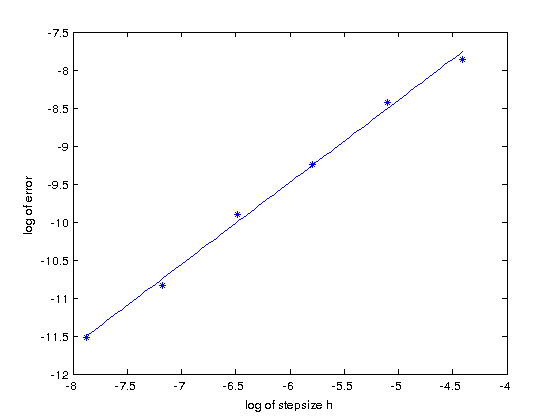
\includegraphics[width=0.8\textwidth]{gfx/loglog}
        \caption{Loglog plog - rate of convergence.}
        \label{fig:loglog}
\end{figure}

\begin{figure}[h]
        \centering
        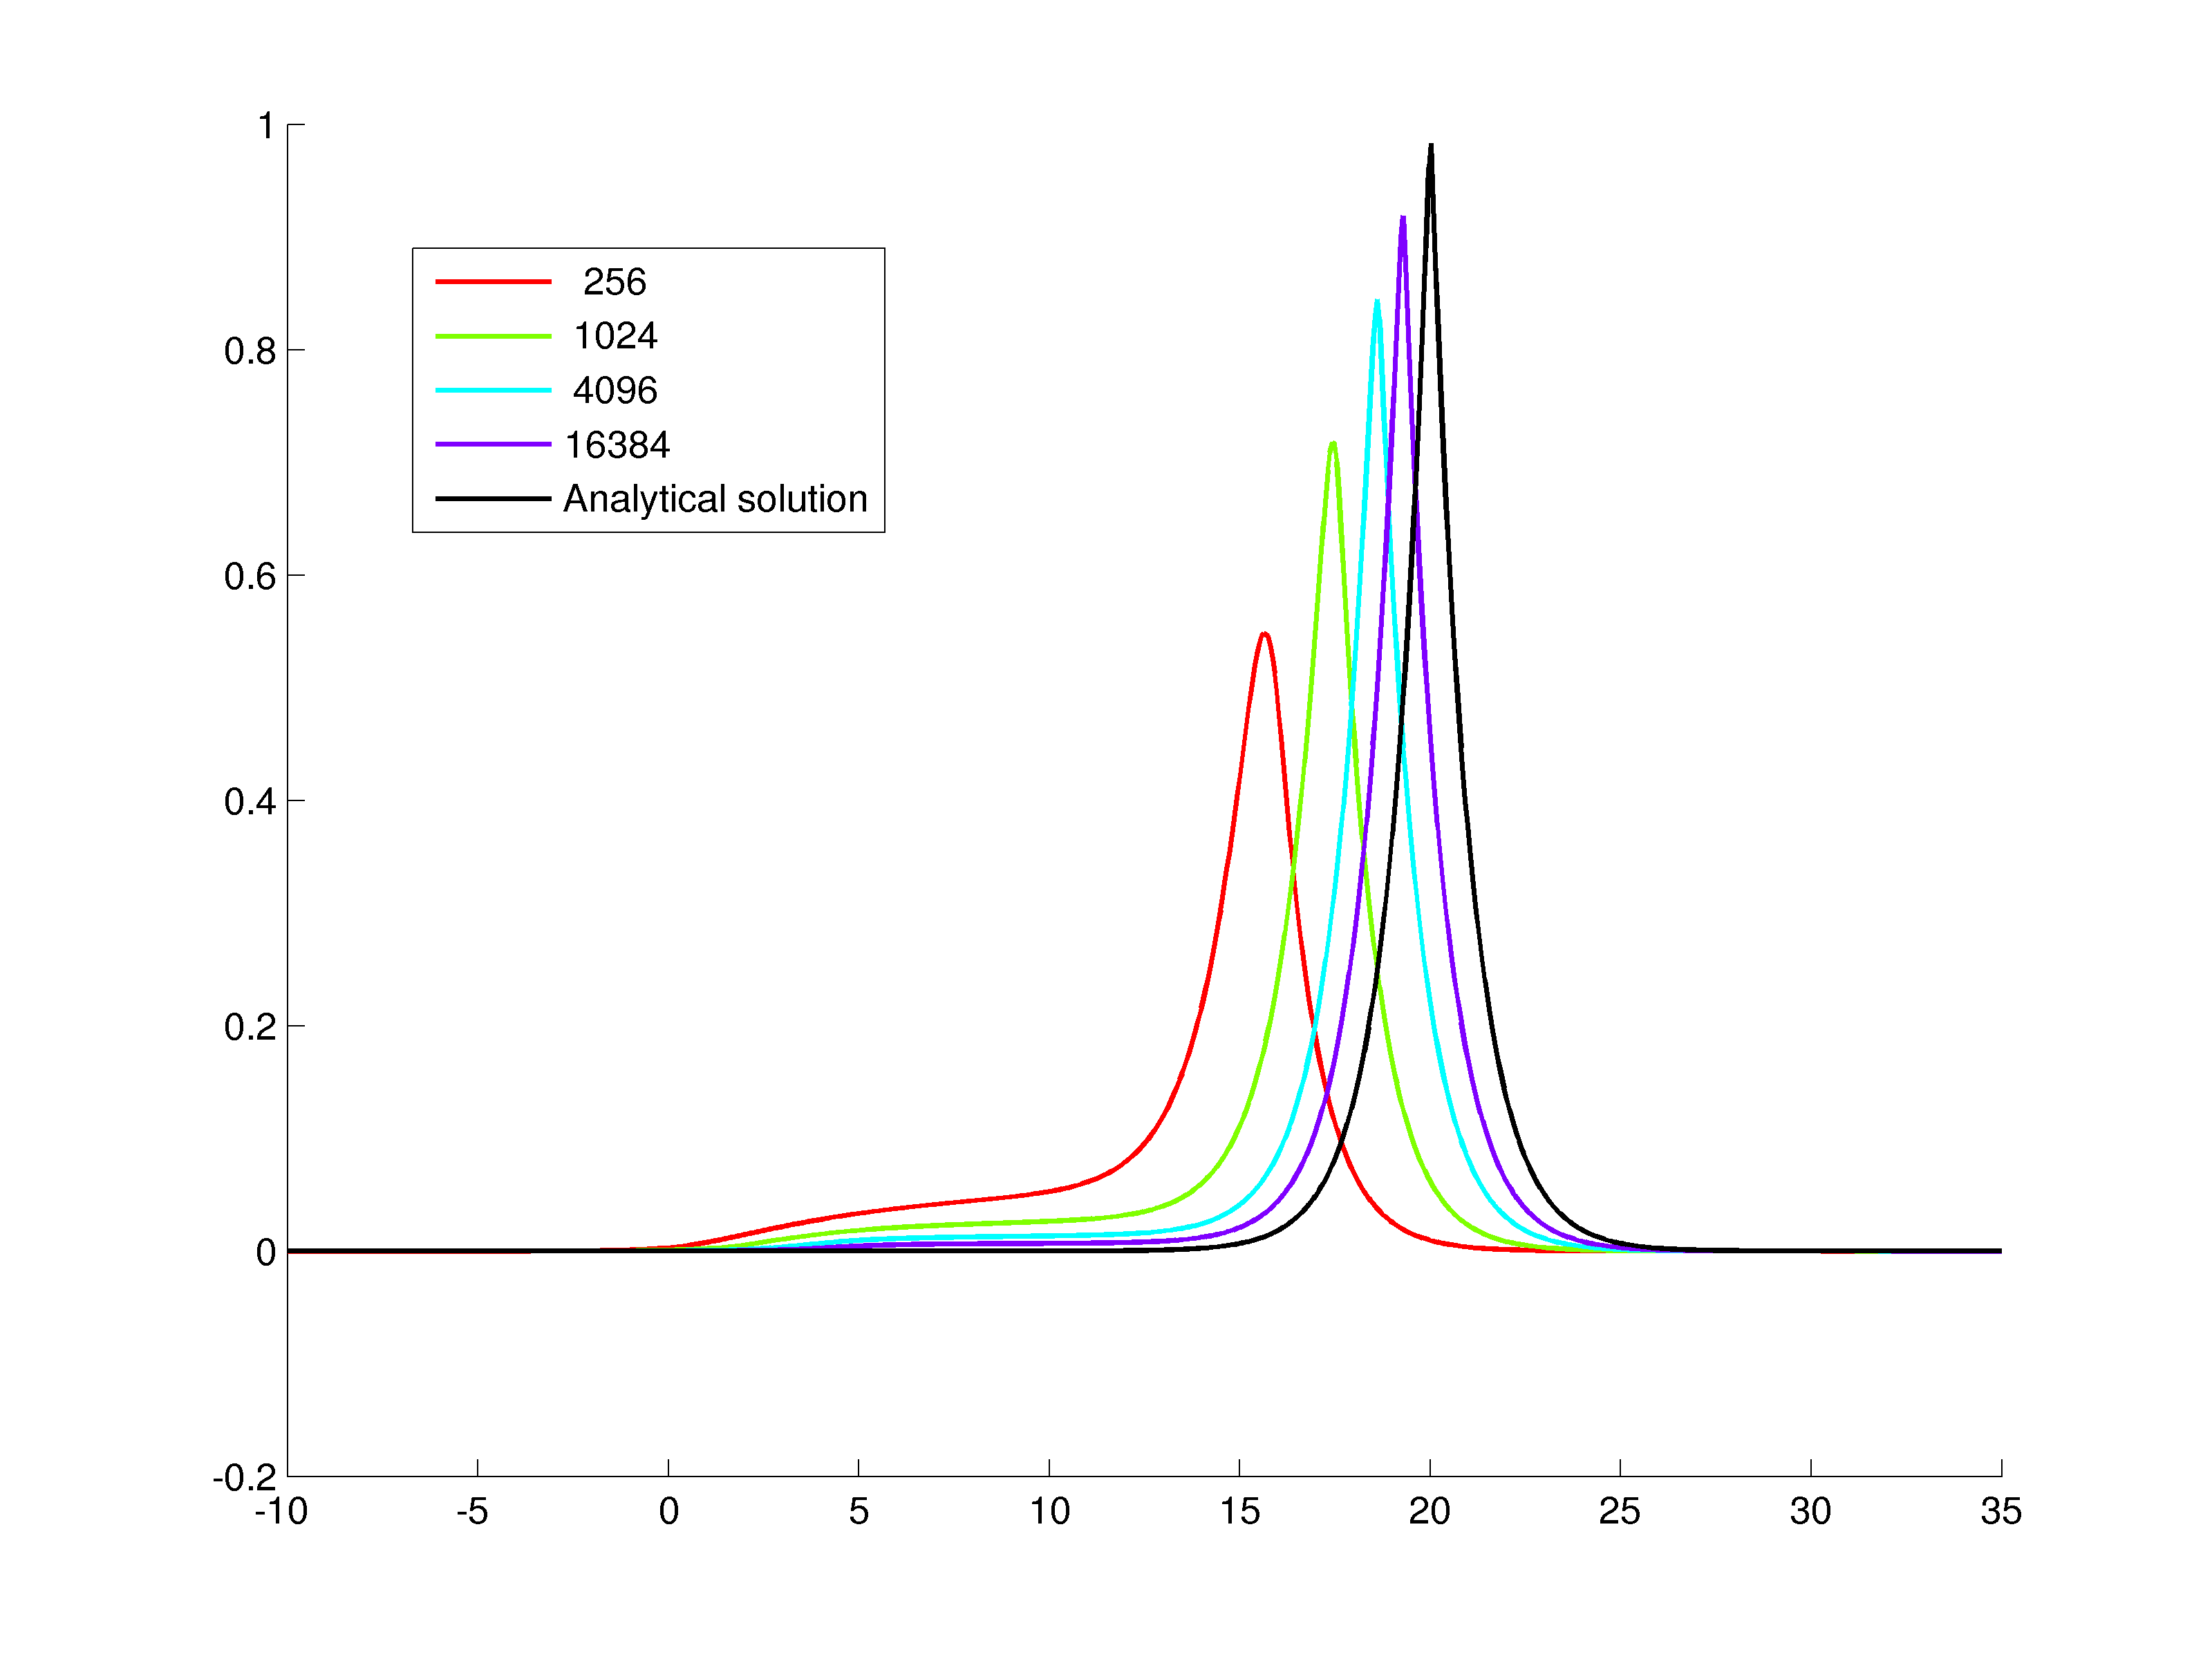
\includegraphics[width=0.8\textwidth]{gfx/attimeT}
        \caption{Plot of approximated solution together with actual solution for decreasing spacial step $h$.}
        \label{fig:attimeT}
\end{figure}

\begin{figure}[h]
        \centering
        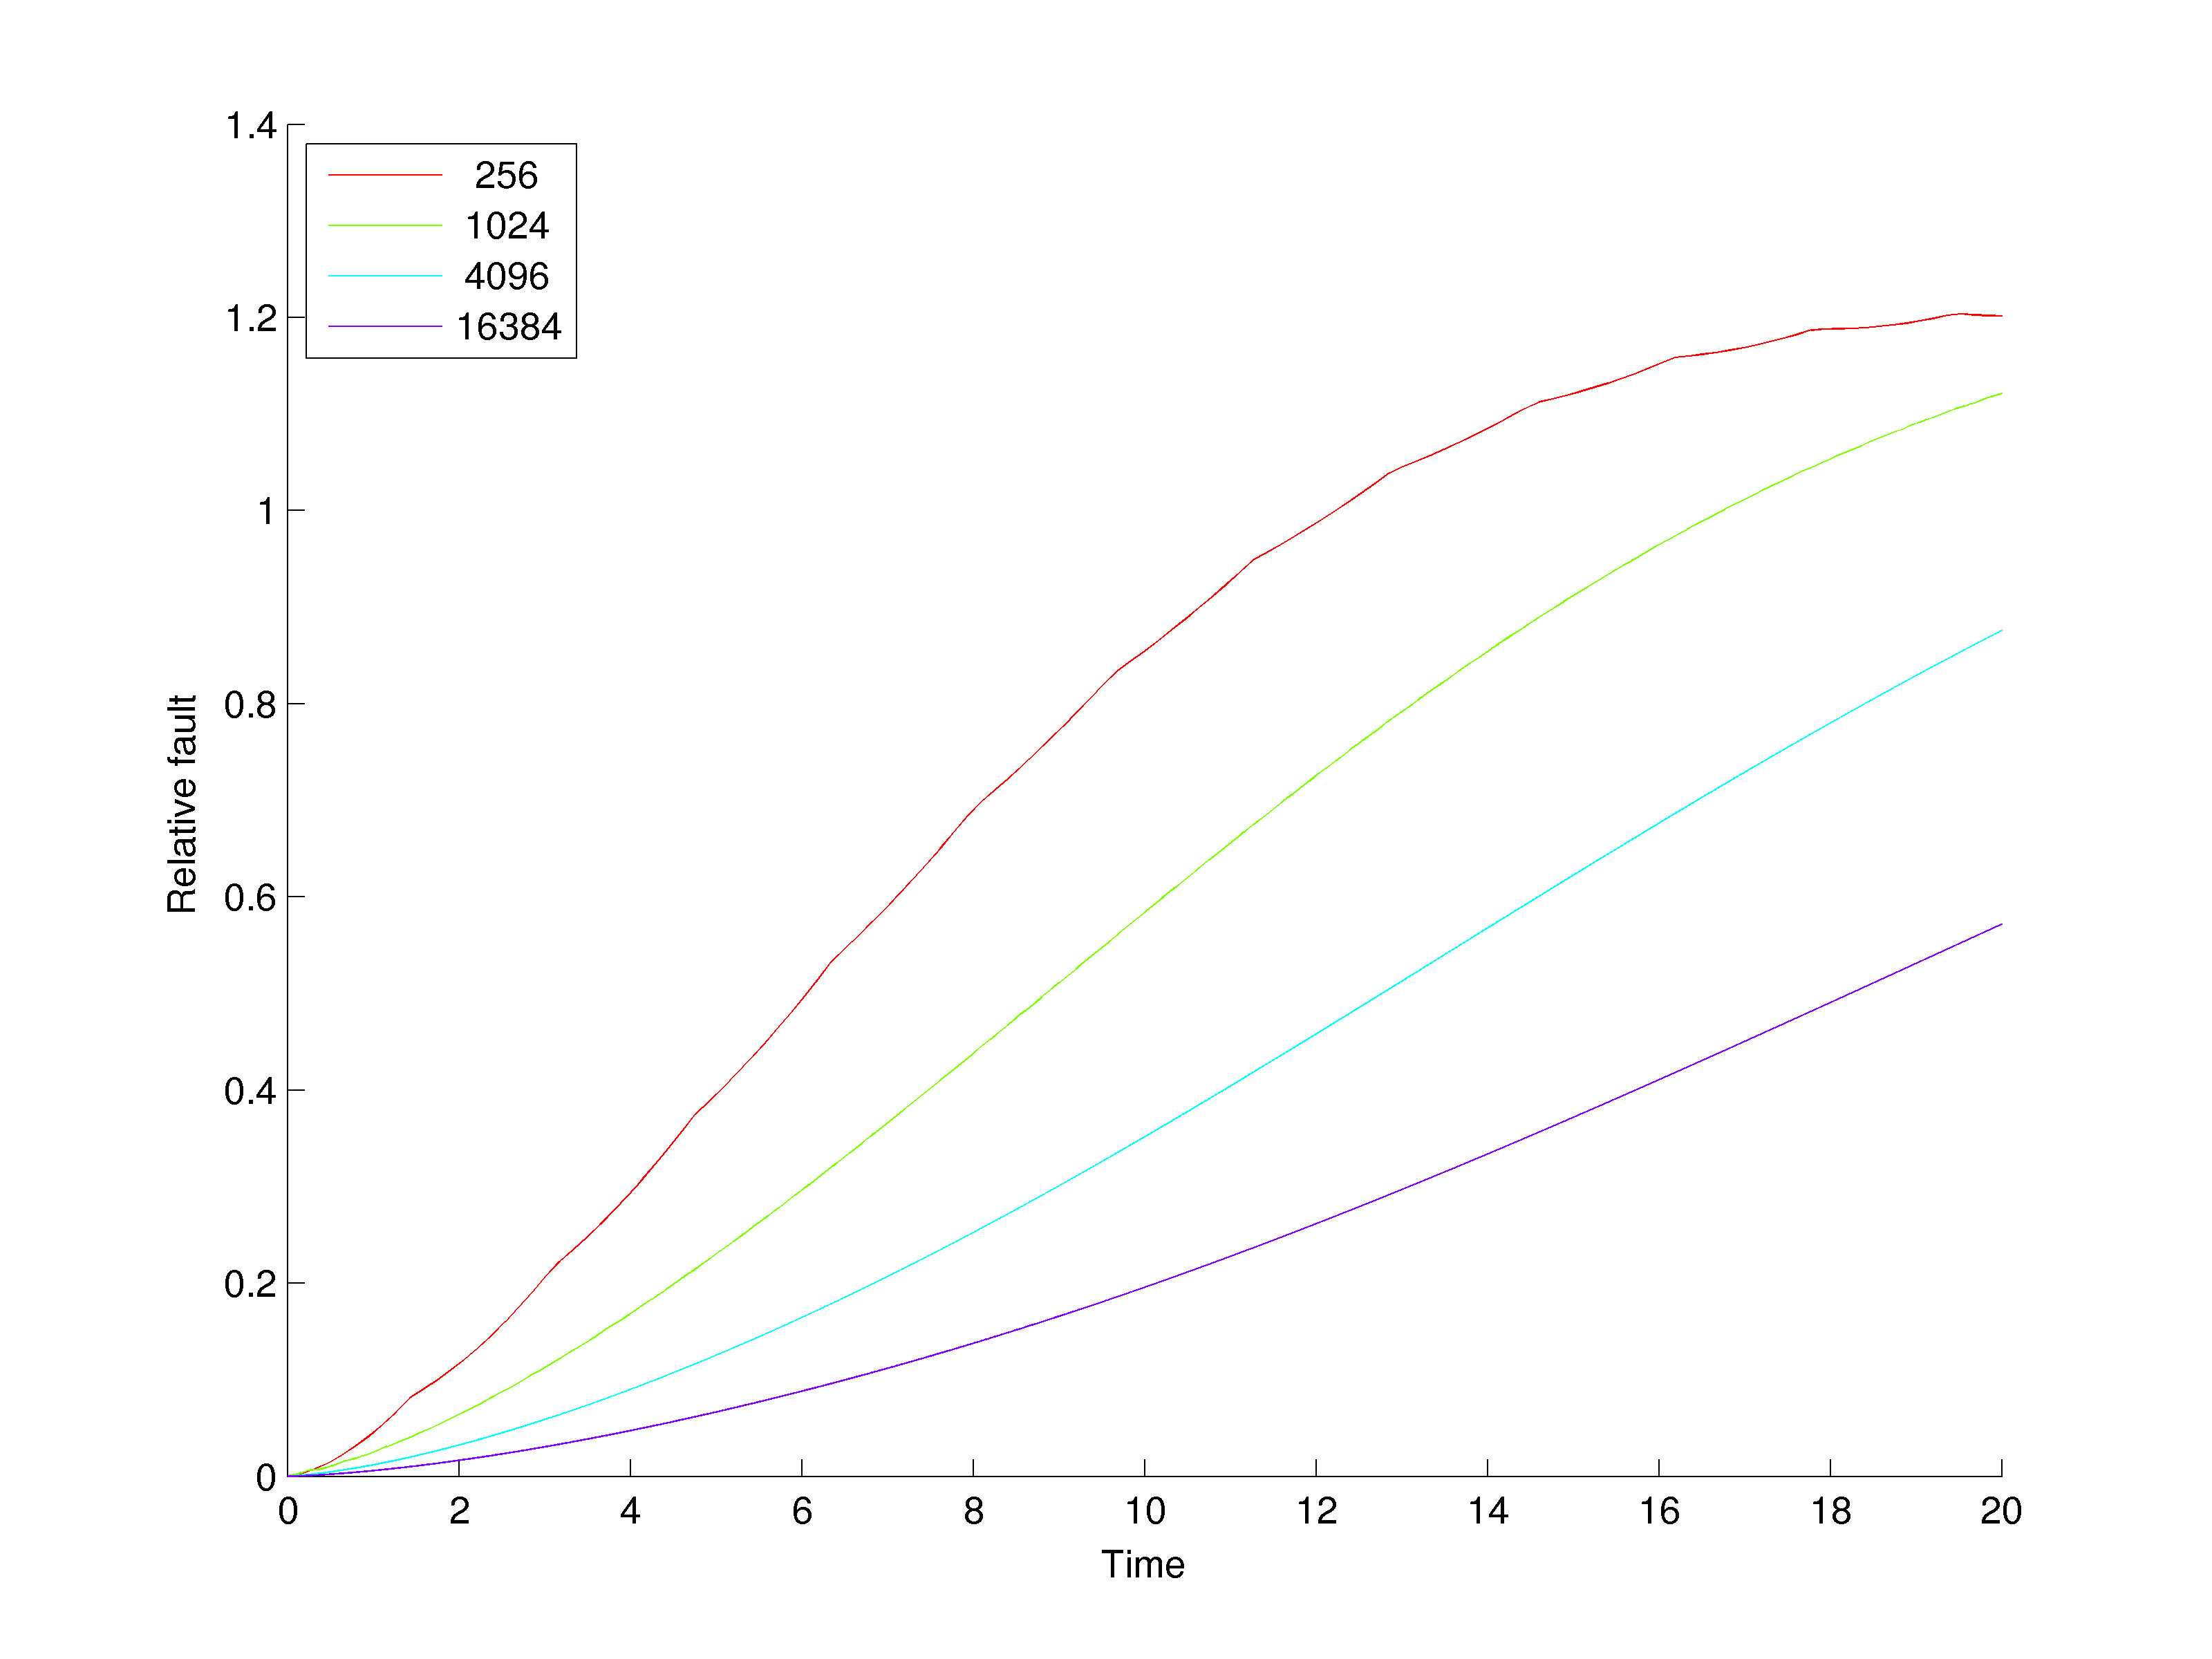
\includegraphics[width=0.8\textwidth]{gfx/erroroftime}
        \caption{Error plots for decreasing $h$, constant time and space interval.}
        \label{fig:erroroftime}
\end{figure}

\subsection*{Semi-discretization}
Writing 
\begin{align*}
m_t = - D_- (m u) - m D u = f(m)
\end{align*},

one may obtain a system of ODEs which can be solved with standard numerical software, though each evaluation of $f$ requires a transformation from $m$ to $u$. Additionally, in the end one needs to transform the resulting matrix of $m$ values back to $u$. Testing a variety of MATLAB's builtin ODE solvers, including \emph{ode45}, \emph{ode15s} and \emph{ode113}, we surprisingly discovered that our explicit scheme based on Euler's method was far superior in every aspect to any other integrator available to us. 

The exact reason why is still unknown to us, though we suspect the discontinuous derivatives of the peakon solutions may cause problems for higher order schemes. This is at least consistent with the fact that the higher order schemes appear to smooth out the peaks of the solution.

Another interesting effect was observed when the timestep of the explicit scheme was decreased (below the bounded value given by our CFL condition) with the spatial step fixed. Numerical experiments suggest that the solution offered by the explicit scheme converges towards the solution of the higher order time integrators as the timestep goes towards zero. In other words, the increased error that results from too small timesteps is somehow bounded by the higher-order schemes. We have not yet been able to discover the cause, and our only hypothesis is at best a farfetched and unlikely guess: perhaps our scheme somehow possesses innate damping, which is inaccurately underestimated by Euler's method in such a way that the explicit scheme experiences less damping than the higher-order integrators?